% Crew Interaction
\section{Crew Interaction}
\begin{frame}{CrewAI Flow}
    \begin{columns}
        \begin{column}{0.45\textwidth}
            \begin{itemize}
                \item Crews coordinate through \textbf{centralized state}
                \item Flow manages \textbf{state} and \textbf{crew kickoffs}
                \item Use of \texttt{\_and}, \texttt{\_or} and \texttt{router} allow \textbf{complex ordering} and \textbf{parallelization}
                \item \textbf{Retry system} facilitates public communications
            \end{itemize}
        \end{column}
        \begin{column}{0.55\textwidth}
            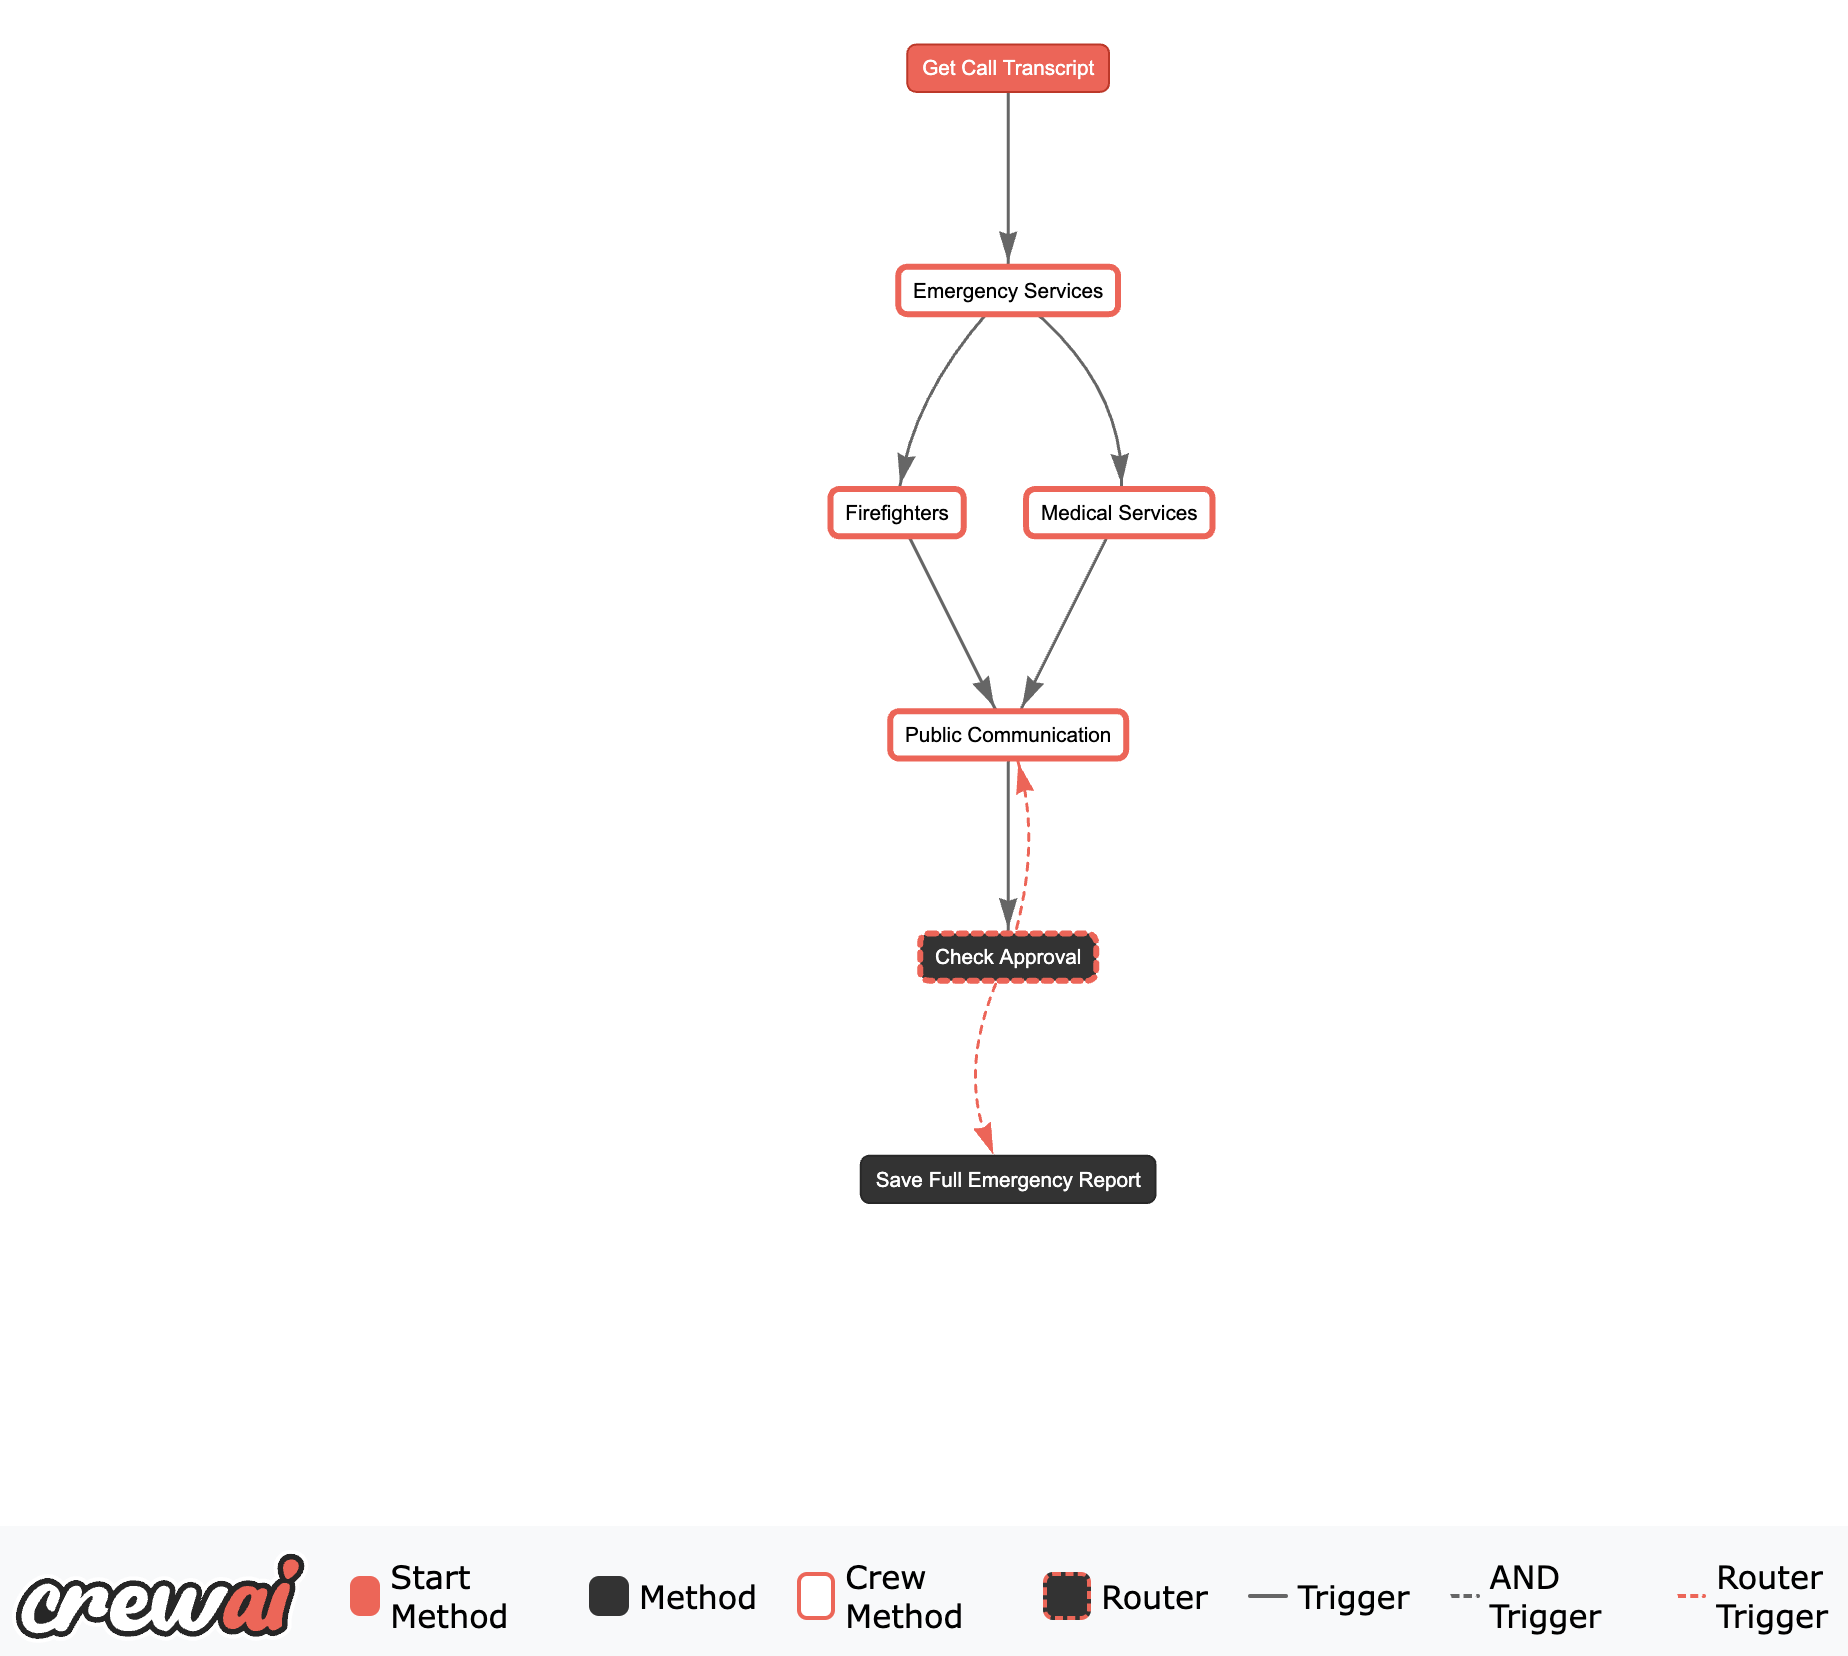
\includegraphics[width=\textwidth]{../figures/coordination_flow.png}
        \end{column}
    \end{columns}
\end{frame}

\begin{frame}[fragile]{Flow State}
    \begin{lstlisting}[language=Python]
class EmergencyPlannerState:
    call_transcript: str | None
    call_assessment: CallAssessment | None
    firefighters_report: FirefightersReport | None
    medical_report: MedicalReport | None
    public_report: PublicReport | None
    retry_count: int = 0
    \end{lstlisting}
\end{frame}